\chapter{Permission management}
\label{chap:ch1}

In order for the application to provide the necessary security over files a permission system
needs to be implemented. There are various ways of implementing permissions, two fairly used 
techniques are Attribute-based access control (ABAC) and Role-based access control (RBAC).
\section{Attribute-based access control}
Attribute-based access control (ABAC) is an authorization model that evaluates attributes 
(or characteristics), rather than roles, to determine access.\cite{keithABAC} The purpose of this 
attribute-based authorization model is to preserve the security and integrity of data 
or devices by restricting access only to authorized users. 

\begin{figure}[htbp]
	\centering
		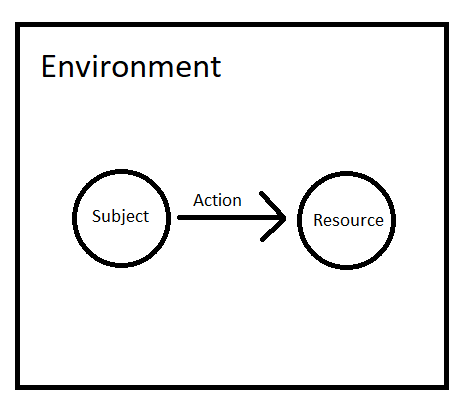
\includegraphics[scale=0.65]{./figures/chapter3/abac.png}
	\caption{The 4 major components of ABAC}
	\label{FigABAC}
\end{figure}


ABAC contains 4 major components: Subject, Resource, Action, and Environment as seen in \ref{FigABAC}.

Although the subject of ABAC is usually associated with a user, in reality,
the Subject can be either a role, a user profile, or essentially any identifying
criteria. Generally, the Subject is identified by their authentication token, 
for example even something like the Personal Numeric Code can be used. 

The Resource is an asset or an object --- be it a file, an application, 
a server or an API --- that the Subject wants to access. 

The Action represents what the Subject wants to perform on the Resource. 
A good example for the Actions is the common actions a file explorer can perform: read, 
write, edit, copy, delete. An Action can have multiple attributes (parameters) 
associated with it. For example, a copy could have the source and the destination.

The Environment represents the context in which the Action has been performed. 
The context can contain data such as: the date and the time when the action was 
performed, the location from which the Subject is trying to perform the Action, 
or even the communication protocol or information about the encryption strength.

Attributes are the characteristics involved during an access event. Attribute-based
access control analyzes these attributes against a set of rules in order to determine
if the subject is authorized.

\subsection*{Advantages}
The key benefit of ABAC is its flexibility. Essentially, the limit for policy-making lies in what attributes must be accounted for, and the conditions the computational language can express. ABAC allows for the greatest breadth of subjects to access the greatest amount of resources without requiring admins to specify relationships between each subject and object. Take the following steps as an example:

\begin{itemize}
    \item When a subject joins an organization, they're assigned a set of subject attributes (e.g., John Doe is a consultant for the radiology department).
    \item An object, when created, is assigned its attributes (e.g., a folder with cardiac imaging test files for heart patients).
    \item  The admin or object owner then creates an access control rule (e.g., "All consultants for the radiology department can view and share cardiac imaging test files for heart patients").
\end{itemize}

Admins can further modify these attributes and access control rules to fit the needs of an organization. For instance, when defining new access policies for external subjects like contractors and providers, they can do so without manually changing each subject-object relationship. ABAC allows for a wide variety of access situations with little administrative oversight.
\subsection*{Disadvantages}
ABAC can be difficult to get off the ground. Admins need to manually define attributes, assign them to every component, and create a central policy engine that determines what attributes are allowed to do, based on various conditions (“if X, then Y”). The model's focus on attributes also makes it hard to gauge the permissions available to specific users before all attributes and rules are in place.\cite{keithABAC}

However, while implementing ABAC can take considerable time and resources, the effort does pay off. Admins can copy and reuse attributes for similar components and user positions, and ABAC's adaptability means that maintaining policies for new users and access situations is a relatively “hands-off” affair.

\section{Role-based access control}

Role-based access control (RBAC) is an authorization model where the roles are the only ways to determine the access to a certain resource or action. A certain simplicity in the ABAC idea is appealing. If a user has attributes that are reflected in the objects they want to access, then access is granted. On the other hand, with RBAC, the permissions granted to a user through roles must be evaluated to determine if the desired access will be granted.\cite{coyneABAC}

\subsection*{Advantages}
Unlike ABAC, where each individual users has a set of attributes, with RBAC all users are assigned a role, which makes the management of the permissions for a set of users easier to manage. Other key benefits of RBAC include:

\begin{itemize}
	\item The possibility of creating a re-assignable sets of permissions.
 	\item Reduce the risk of human error when assigning permissions. 
  	\item Granularity of permissions is still preserved by breaking up permissions into multiple roles and assigning multiple roles to users.
	\item Reduce administrative work by having the possibility of quickly changing the user's roles (i.e after a project ends and an user access needs to be revoked).
 	\item Decrease the security risks by restricting access to sensitive information in a more controlled manner.
\end{itemize}

\subsection*{Disadvantages}
Despite having a simpler implementation compared to ABAC, RBAC does of course come with disadvantages. The main disadvantage of RBAC is that due to the increasing number of different roles, managing said roles becomes a very complex task if the management wishes to have properly encapsulated permissions.

Granularity is also much harder to achieve than with an ABAC system. In the case where you want only a user to have a privilege and that user is part of a group already, the only way to give that user and only that user the privilege is to create a new role solely for that.